\documentclass[border=6pt]{standalone}
\usepackage{tikz}
\usepackage{pgfplots}
\pgfplotsset{compat=1.18}
\usetikzlibrary{arrows.meta,positioning,shapes.geometric,fit,backgrounds,calc,decorations.pathreplacing,patterns,pgfplots.groupplots}
\tikzset{
  blk/.style={rectangle, rounded corners=2pt, draw=black!70, thick, fill=blue!6,
              minimum height=8mm, minimum width=20mm, align=center, font=\small},
  io/.style={rectangle, rounded corners=6pt, draw=black!70, thick, fill=green!8,
             minimum height=8mm, align=center, font=\small},
  proc/.style={rectangle, draw=black!70, thick, fill=orange!10, minimum height=8mm,
               align=center, font=\small},
  dec/.style={diamond, aspect=2, draw=black!70, thick, fill=yellow!15, align=center, font=\footnotesize},
  warnbox/.style={rectangle, rounded corners=2pt, draw=red!60!black, thick, fill=red!7,
                  minimum height=8mm, align=center, font=\small},
  oklbox/.style={rectangle, rounded corners=2pt, draw=green!45!black, thick, fill=green!8,
                 minimum height=8mm, align=center, font=\small},
  ar/.style={-{Latex[length=2mm]}, thick},
  arl/.style={-{Latex[length=2mm]}, thick, dashed, draw=black!55},
  lbl/.style={font=\footnotesize\itshape, text=black!60},
}
\definecolor{good}{RGB}{34,139,34}
\definecolor{bad}{RGB}{178,34,34}
\definecolor{warn}{RGB}{218,165,32}
\definecolor{pesblue}{RGB}{0,45,98}
\definecolor{complete}{RGB}{30,125,79}
\definecolor{partial}{RGB}{176,106,0}
\definecolor{blocked}{RGB}{166,43,43}
%% ---- figure-local styles (the wrapper above is unchanged) ----
\tikzset{
  panel/.style={font=\small\bfseries, text=pesblue},
  runlbl/.style={font=\footnotesize\bfseries, text=black!75},
  dim/.style={blk, draw=black!35, thin, fill=black!9, text=black!50,
              minimum width=32mm, text width=28mm, inner sep=2pt},
  hi/.style={blk, draw=pesblue, very thick, fill=blue!18, text=black,
             minimum width=32mm, text width=28mm, inner sep=2pt,
             font=\small\bfseries},
  sl/.style={rectangle, rounded corners=2pt, draw=black!60, thick, fill=white,
             minimum height=6mm, minimum width=24mm, text width=21mm,
             align=center, font=\scriptsize, inner sep=1.5pt},
  sldiff/.style={sl, draw=bad, very thick, dashed, fill=red!7},
  vok/.style={oklbox, draw=complete, text=complete, text width=38mm},
  vbad/.style={warnbox, draw=blocked, text=blocked, text width=54mm},
  dlab/.style={lbl, text=bad, anchor=west, align=left, text width=1.9cm},
  glab/.style={lbl, anchor=west, align=left, text width=1.9cm},
}
\begin{document}
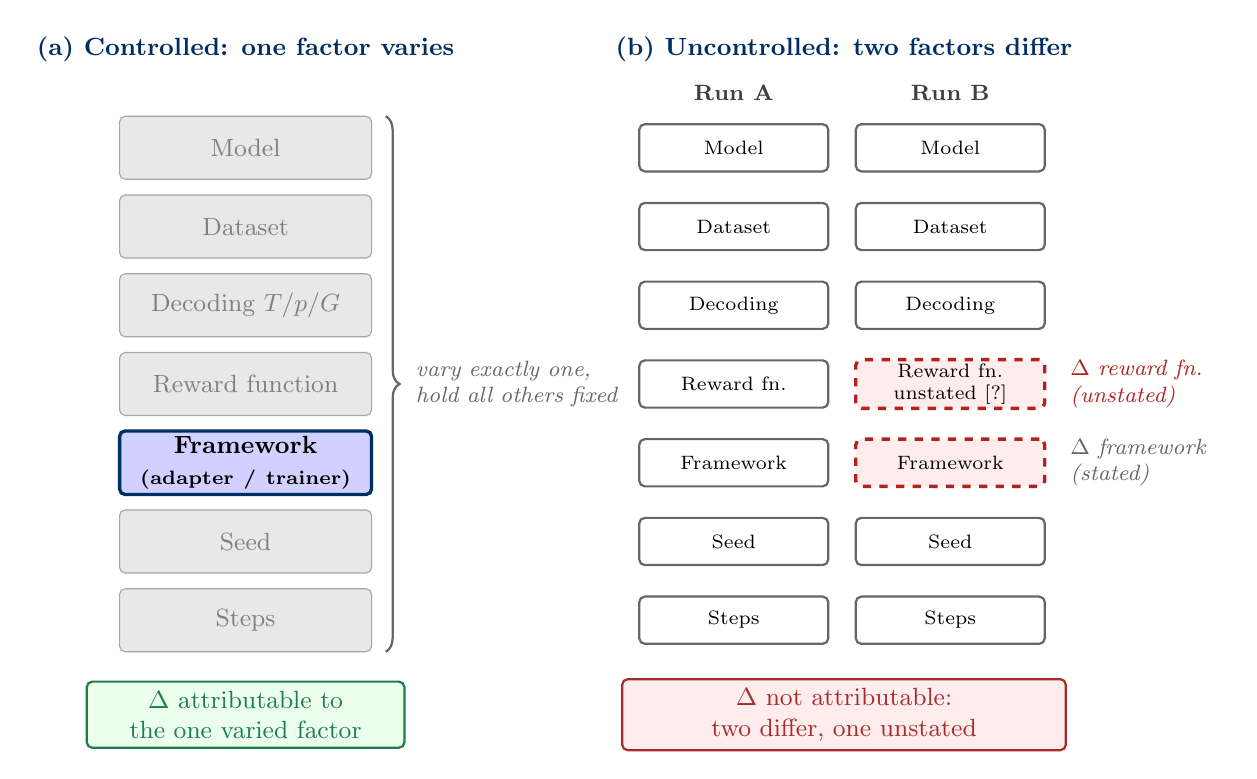
\begin{tikzpicture}

%% =====================================================================
%% (a) Controlled: one component of the stack is varied, rest held fixed
%% =====================================================================
\node[panel] at (0,1.25) {(a) Controlled: one factor varies};

\node[dim] (a1) at (0, 0.0) {Model};
\node[dim] (a2) at (0,-1.0) {Dataset};
\node[dim] (a3) at (0,-2.0) {Decoding $T/p/G$};
\node[dim] (a4) at (0,-3.0) {Reward function};
\node[hi]  (a5) at (0,-4.0) {Framework\\{\scriptsize (adapter / trainer)}};
\node[dim] (a6) at (0,-5.0) {Seed};
\node[dim] (a7) at (0,-6.0) {Steps};

%% brace over the whole stack: exactly one varies, the rest are pinned
\draw[decorate, decoration={brace, amplitude=5pt}, draw=black!60, thick]
  (1.78,0.40) -- (1.78,-6.40);
\node[lbl, anchor=west, align=left, text width=2.78cm] at (2.04,-3.0)
  {vary exactly one,\\ hold all others fixed};

\node[vok] at (0,-7.20) {$\Delta$ attributable to\\the one varied factor};

%% =====================================================================
%% (b) Contrast: two runs that differ in more than one component,
%%     one of which was never stated, cannot be attributed
%% =====================================================================
\node[panel] at (7.6,1.25) {(b) Uncontrolled: two factors differ};
\node[runlbl] at (6.2,0.70) {Run A};
\node[runlbl] at (8.95,0.70) {Run B};

%% --- Run A: a fully stated stack ---
\node[sl] (b1) at (6.20, 0.0) {Model};
\node[sl] (b2) at (6.20,-1.0) {Dataset};
\node[sl] (b3) at (6.20,-2.0) {Decoding};
\node[sl] (b4) at (6.20,-3.0) {Reward fn.};
\node[sl] (b5) at (6.20,-4.0) {Framework};
\node[sl] (b6) at (6.20,-5.0) {Seed};
\node[sl] (b7) at (6.20,-6.0) {Steps};

%% --- Run B: framework differs as intended, reward fn. differs unstated ---
\node[sl] (c1) at (8.95, 0.0) {Model};
\node[sl] (c2) at (8.95,-1.0) {Dataset};
\node[sl] (c3) at (8.95,-2.0) {Decoding};
\node[sldiff] (c4) at (8.95,-3.0) {Reward fn.\\unstated [?]};
\node[sldiff] (c5) at (8.95,-4.0) {Framework};
\node[sl] (c6) at (8.95,-5.0) {Seed};
\node[sl] (c7) at (8.95,-6.0) {Steps};

%% callouts on the two differing components
\node[glab] at (10.35,-4.0) {$\Delta$ framework\\(stated)};
\node[dlab] at (10.35,-3.0) {$\Delta$ reward fn.\\(unstated)};

\node[vbad] at (7.60,-7.20) {$\Delta$ not attributable:\\two differ, one unstated};

\end{tikzpicture}
\end{document}
